\documentclass{article} % For LaTeX2e
\usepackage{iclr2018_conference,times}
\usepackage{hyperref}
\usepackage{url}
\usepackage[pdftex]{graphicx}
\usepackage{subfigure}
\usepackage{wrapfig}
\usepackage{amssymb}


%\title{Automated Aerodynamic Design using Neural Networks and Gradient Decent}
\title{Automated Design using Neural Networks and Gradient Decent}

% Authors must not appear in the submitted version. They should be hidden
% as long as the \iclrfinalcopy macro remains commented out below.
% Non-anonymous submissions will be rejected without review.

\author{Oliver Hennigh \\
Mexico\\
Guanajuato, Gto, Mexico \\
\texttt{loliverhennigh101@gmail.com} \\
}

% The \author macro works with any number of authors. There are two commands
% used to separate the names and addresses of multiple authors: \And and \AND.
%
% Using \And between authors leaves it to \LaTeX{} to determine where to break
% the lines. Using \AND forces a linebreak at that point. So, if \LaTeX{}
% puts 3 of 4 authors names on the first line, and the last on the second
% line, try using \AND instead of \And before the third author name.

\newcommand{\fix}{\marginpar{FIX}}
\newcommand{\new}{\marginpar{NEW}}

\iclrfinalcopy % Uncomment for camera-ready version, but NOT for submission.

\begin{document}


\maketitle

\begin{abstract}

We propose a novel method that makes use of deep neural networks and gradient decent to perform automated design on complex real world engineering tasks. Our approach works by training a neural network to mimic the fitness function of a design optimization task and then, using the differential nature of the neural network, we perform gradient decent to maximize the fitness. We demonstrate this methods effectiveness by designing an optimized heat sink and both 2D and 3D airfoils that maximize the lift drag ratio under steady state flow conditions. We highlight that our method has two distinct benefits over other automated design approaches. First, evaluating the neural networks prediction of fitness can be orders of magnitude faster then simulating the system of interest. Second, using gradient decent allows the design space to be searched much more efficiently then other gradient free methods. These two strengths work together to overcome some of the current shortcomings of automated design.

\end{abstract}

\section{Introduction}

Automated Design is the process by which an object is designed by a computer to meet or maximize some measurable objective. This is typically performed by modeling the system and then exploring the space of designs to maximize some desired property whether that be an automotive car styling with low drag \cite{ando2010automotive} or power and cost efficient magnetic bearings \cite{dyck1996automated} . A notable historic example of this is the 2006 NASA ST5 spacecraft antenna designed by a evolutionary algorithm to create the best radiation pattern \cite{hornbyautomated}. More recently, an extremely compact broadband on-chip wavelength demultiplexer was design to split electromagnetic waves with different frequencies \cite{piggott2015inverse}. While there have been some significant successes in this field the dream of true automated is still far from realized. The main challenges present are heavy computational requirements for accurately modeling the physical system under investigation and often exponentially large search spaces. These two problems negatively complement each other making the computation requirements intractable for even simple problems. For example, in the flow problems explored in this work, a heavily optimized flow solver running on modern GPU requires around 3 minutes to perform each simulation. Given that as many as 3,000 designs may need to be tested to find one with reasonable performance, this results in a total computation time of 9 days. Increasing the resolution of the simulation or expanding the parameter space quickly make this an unrealizable problem without considerable resources.

Our approach works to solve the current problems of automated design in two ways. First, we learn a computationally efficient representation of the physical system on a neural network. This trained network can be used to evaluate the quality or fitness of the design several orders of magnitude faster. Second, we use the differentiable nature of the trained network to get a gradient on the parameter space when performing optimization. This allows significantly more efficient optimization requiring far fewer iterations then other gradient free methods such as genetic algorithms or simulated annealing. These two strengths of our method overcome the present difficulties with automated design and allow the previous mention 9 day optimization to run in only 10 minutes. 

The first problem tackled in this work is designing a simple heat sink to maximize the cooling of a heat source. The setup of our simulation is meant to somewhat mimic the conditions seen with an aluminum heat sink on a computer processor. We keep this optimization problem relatively simple though and use this only as a first test and introduction to the method. Our second test is on the significantly more difficult task of designing both 2D and 3D airfoils with high lift drag ratios under steady state flow conditions. This problem is of tremendous importance in many engineering areas such as aeronautical, aerospace and automotive engineering. Because this is a particularly challenging problem and often times unintuitive for designers, there has been considerable work using automated design to produce optimized designs. We center much of the discussion in this paper around this problem because of its difficulty and view this as a true test our method. While we only look at these two problems in this work, we emphasize that the ideas behind our method are applicable to a wide variety of automated design problems.

As we will go into more detail in later sections, in order to perform our flow optimization tests we need a network that predicts the steady state flow from an objects geometry. This problem has previously been tackled in \citep{guo2016convolutional} where they use a relatively simple network architecture. We found that better perform could be obtained using some of the modern network architecture developments and so, in addition to presenting our novel method of design optimization, we also present this superior network for predicting steady state fluid flow with a neural network.

This work has the following contributions.
\begin{itemize}
  \item We demonstrate a novel way to use neural networks to greatly accelerate automated design.
  \item We present this method in such a way that it can ready applied to many other automated design problems by demonstrating its use on two vastly different design tasks.
  \item We provide a new network architecture for predicting steady state fluid flow that vastly out performs previous models.
\end{itemize}

\section{Related Work}

Because this work is somewhat multidisciplinary, we give some background information on the different areas. In particular, we provide a brief discussion of other work related to emulating physics simulations with neural networks as this is of key importance in our method. We also review some of the prior work in automated design of airfoils because this is the main problem used to test our method.

\section{Speeding up Computational Physics with Neural Networks}

In recent years there has been incredible interest in applications of neural networks to computational physics problems. One of the main pursuits being to emulate the desired physics for less computation then the physics simulation. Example applications range from simulating 3D high energy particle showers seen in \citep{2017arXiv170502355P} to solving the Schrödinger equation seen in \citep{mills2017deep}. Computational Fluid Dynamics has gotten the most attention in this regard because of its many uses in engineering as well as computer animation \cite{tompson2016accelerating} \cite{2017arXiv170509036H}. The prior work that is most related to our own is \citep{guo2016convolutional} where they train a neural network to predict the steady state fluid flow from an objects geometry. Our method builds on this idea and we use the same general approach for approximating the fluid flow but with and improved architecture.

\subsection{Automated Design Optimization of Airfoils}

To date, there has been substantial work in automated aerodynamic design for use in aeronautical and automotive applications \cite{ando2010automotive} \cite{demultiplexer}. Airfoil optimization in particular has received a lot of attention where the general methodology is to refine an airfoil geometry to maximize the lift drag ratio \cite{drela1998pros}. Roughly speaking, there are two classes of optimization strategies used here. The first class being gradient free methods like simulated annealing, genetic algorithms, and particle swarm methods. A look at these methods and there applications to airfoil optimization can be found here \cite{mukesh2012application}. The other class being gradient based methods like steepest decent and quasi-newtonian methods. Typically gradient based methods can perform optimization in fewer steps then gradient free methods however computing the gradient is often very costly. The simplest approach in doing so is finite difference method however this requires simulating the system a proportional number of times to the dimension of the search space to approximate the gradient. This is infeasible if the fluid simulation is computationally expensive. Another approach is the adjoint method however. Our approach can be viewed as one of these gradient based methods but where the gradients are coming from a neural network that is emulating the simulation.

In order to perform automated design of airfoils one needs to parameterize the space of possible geometries. There are a variety of approaches in doing this and a thorough list can be found here \cite{salunke2014airfoil}. In this work we use the parameterization technique found in \cite{lane2009surface} and \cite{hilton2007universal} where the upper and lower surface are described by a polynomial and the parameters are the coefficients of this polynomial.

\section{Gradient Decent on Parameter Space}

\begin{figure}[h]
\begin{center}
%\framebox[4.0in]{$\;$}
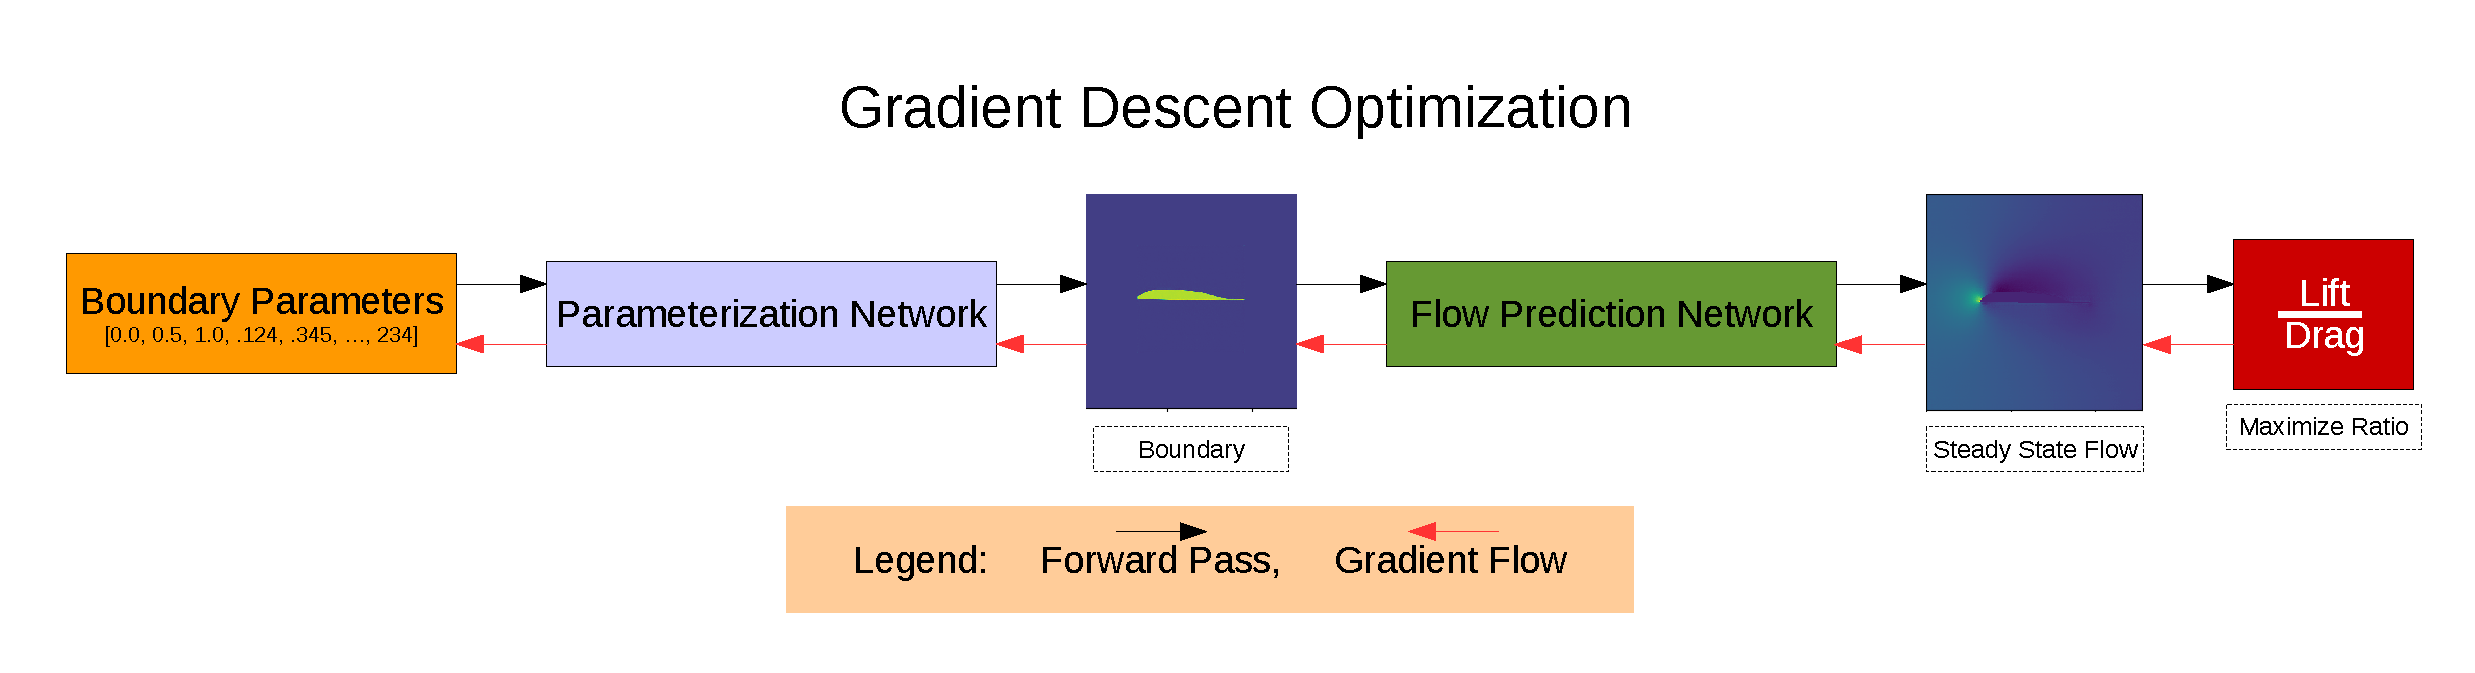
\includegraphics[scale=0.34]{./gradient_descent_optimization.pdf}
%\fbox{\rule[-.5cm]{0cm}{4cm} \rule[-.5cm]{4cm}{0cm}}
\label{gradient_descent_optimization}
\end{center}
\caption{Illustration of Proposed Gradient Decent Method}
\end{figure}


Our automated design optimization problem can be viewed in concrete terms as maximizing some desired fitness function $F(x)$, where $F:X \rightarrow \mathbb{R}$ for some space $X$ of design parameters.

\begin{equation}
  \max_{\forall x \in X} F(x)
\end{equation}

In most real world setting, evaluating the fitness function $F$ can be computationally demanding as is the case with our fluid simulations. The first aspect of our method is to replace $F$ with a computationally efficient neural network $F_{net}$. This can offer considerable speed improvements as we will discuss bellow. The second piece of our method is the observation that $F_{net}$ is differentiable and can be used to obtain a usable gradient in the direction of maximizing fitness. This is in contrast to $F$ where it may be computationally infeasible to calculate the gradient and thus require other search techniques such as simulated annealing or genetic algorithms. Using this gradient allows faster optimization to be performed with fewer iterations as we will demonstrate bellow. There are some details that need to be addressed though and to do this we go through the example problem of optimizing the fin heights on a heat sink.

In our simple heat sink problem, $X$ contains 15 real valued parameters between 0 and 1. Each of these parameters corresponds to the height of an aluminum fin on the heat sink as seen in the figure \ref{heat_sink_optimization}. In this optimization problem we fix the amount of aluminum and scale the total length of all the fins to meet this requirement. This presents an interesting problem of determining the optimal length each fin should have to maximize the cooling of the heat source. The simplest application of our method is use the 15 fin heights as inputs to a neural network that outputs a single value corresponding to the temperature at the heat source. This approach has the draw back that if you want to add another constraint to the optimization like making the left side is cooler then the right side you would need to retrain the network. A solution to this is to have the network again take in the fin parameters but output the full heat distribution of the heat sink. This allows different quantities to be optimized but is still limiting in that our network only runs on a single parameter set up. Our solution to this problem is to train two networks. The first network, $P^{heat}_{net}$, takes in the fin parameters and generates a binary image corresponding to the geometry of the heat sink. We refer to this as the parameterization network. The second network, $S^{heat}_{net}$, predicts the steady state heat distribution from the geometry. Because the parameterization network is performing an extremely simple task and training data can be generating cheaply, we can quickly retrain $P^{heat}_{net}$ if we want to change the parameter space. The network $S^{heat}_{net}$ is now learning the more general task of predicting steady state heat flow on an arbitrary geometry. The same approach is used for the steady state flow problem and a figure depicting this can be found \ref{gradient_descent_optimization} . This approach allows our network to be as versatile as possible while still allowing it to used on many design optimization tasks.

Up until now we have not discussed how to generate data needed to train these neural networks. Generating the data to train the parameterization network is relatively simple. If the parameterization is known, we simply make a set of parameter vectors and there corresponding geometries. In the case of the heat sink this is a set of examples composed of the 15 parameters and there corresponding binary representation of the head sink. Putting together a dataset for $S^{heat}_{net}$ or $S^{flow}_{net}$ (fluid flow network) is somewhat more complex. The simplest approach and the one used in this work is to simulate the respective physics on objects drawn from the object design space. For the heat sink problem this would entail a dataset of object geometries and their corresponding steady state heat distributions. This method has the disadvantage that the network only sees examples from the current parameter search space and if it is changed the network may not be able to accurately predict the physics. We argue this is not a significant issue for several reasons. First, in the work seen here the network is able to generalize effectively to objects well outside its train set. During the course of this work we tested our network on a variety of datasets and found similar generalizable abilities. Second, it is easy to imagine a system where a network is trained on a large set of diverse simulations and then fine tuned on the current desired parameter space when desired. For these reasons we feel that this approach of generating simulation data is not significantly limiting and does not distract from the generalizability of the approach.

\subsection{Flow Prediction Network}

The core component of our method is being able to emulate the physics simulation with a neural network. For the steady state flow problem here has already been work doing just this found here. As mentioned above, we have made some improvements to this network architecture design and training. A figure illustrating our network can be found here. This model resembles the U-network architecture seen here with a series skip after each down sample. The advantages of this style of network are its high performance on image to image type tasks, trainability on small datasets, and fast evaluation time in comparison to networks with large fully connected layers. The trainability on small datasets make this particularly effective on predicting steady state flow because generating simulation data to train on is time consuming. Our network is able to train on relatively small datasets of only 4,000 flow simulation in comparison to the 100,000 required in previous work predicting steady state flow. Other modifications we have used are the use of gated residual blocks blocks that allow the gradient to be propagated extremely efficiently and heavily lowers training time.

\section{Experiments}

%In the following sections we subject our method and model to a variety of test in order to see its performance. Because our method is centered around gradients oThe goal being first to determine how accuraty and fast our model can predict steady state flow. In particular, what its accuracy in predicting values such a drag and lift as these are important quantitize in our optimization. Second, we investigate how effective our gradient decent optimization is. This line of tests compares our method to other none gradient based search techniques and illustrates what is happening in the optimization processes looks like. For example, what does the gradient surface look like.

\subsection{Datasets}

To train the parameterization networks we generated a set of 10,000 examples for each system consisting of a parameter vector and their corresponding geometry. The 

The heat sink simulations dataset consists of BLANK training examples simulated with implicit finite difference method.

\subsection{Training}

For all networks we used the Adam optimizer \cite{kingma2014adam}. For $S^{heat}_{net}$ or $S^{flow}_{net}$ a learning rate of 1e-4 was used until the loss platued and then the learning rate was dropped to 1e-5. Mean Squared Error was used as the loss function however when training the flow prediction network we scaled up the loss from the pressure field by a factor of 30 to roughly match the magnitude of the velocity vector field. Without this modification the network would only learn the pressure field once the velocity vector field was firmly learned. During the course of this work other loss functions were experimented with. In particular, we tried adding a loss term in predicting the fluid flow forces on the object. This had the beneficial effect of higher accuracy in predicting forces but complicated the method and was too specific to fluid flow to justify. The parameterization networks also used Mean Squared Error with a constant learning rate of 1e-4. We found the parameterization networks trained extremely quickly.

\subsection{Gradient Decent Design Optimization Details}

There are some complexities in how exactly to the design parameters are optimized that need explanation. When training the parameterization network, the raw design parameters are used from there respective ranges and sent through the network. During design optimization however, the trainable design parameters go through a hard sigmoid functions and then are scaled to there appropriate range before being sent through the parameterization network. This is done to ensure the parameters being searched are within the range but also presents a challenge because if the parameters leave the range -1 and 1 the gradient will go to zero and they will be stuck at that value for the duration of the optimization. We overcame this problem by placing a small loss on any parameter greater then 1 or less then -1. This prevents the parameters from getting stuck and allows mobility for the entire optimization process.

One expected difficulty in optimizing the parameters is falling into local optima. In later sections we will go into more detail about what the gradients look like in the search space but for right now we will proscribe a simple solution of using gradient decent with momentum. For all the experiments we used this technique with learning rate blaa and momentum blaa. We also found that adding a small amount of noise to the parameters helped get out of bad gradient positions as well. This has the effect of somewhat smoothing the gradient around its space.

\subsection{Heat Sink Optimization}

As discussed above, the heat sink optimization task is to find a set of fin heights that maximally cool a constant heat source given a fixed total length of the fins. The set up roughly corresponds to an aluminum heat sink placed placed on a CPU where the heat source is treated as an addition of temperature. There is no heat dissipation between the underside of the heat sink but all other areas not on the heat sink are kept at a constant temperature. The heat diffusion constant in the heat sink is kept at 1000 and the diffusion constant at the boundary is 10. The intuitive solution to this optimization problem is to place long fins near the heat source and shorter fins farther away. Balancing this is a difficult task though because changing the length of any fin has a global effect on how much heat is dissipated by all the other fins. 

After training our networks $P^{heat}_{net}$ and $S^{heat}_{net}$ we perform our proposed gradient optimization on the 15 fin heights to minimize the temperature at the source. In figure \ref{heat_sink_optimization} we see the optimized heat sink and see that the design resembles what our intuition tells us. We also not the extremely smooth optimization that occurs with only small bumps caused by the small addition of noise noted above. A natural question to ask is how this compares to other search techniques and how closely this optimized design resembles the true best design. In order to answer these questions we use simulated annealing to search designs and use the original heat diffusion solver to evaluate their performance. In figure blank we see that the heat optimized heat sink design produced by the neural network closely resembles that produces by a simulated annealing. There are some minute differences however the total effectiveness in cooling the system are almost identical. We also note the incredible speed difference between the two methods. The gradient decent approach required roughly 300 iterations to converge where as the simulated annealing approach needed 600. In real time the gradient decent required approach took 2.3 seconds on a Nvidia 1070 gtx GPU and the simulated annealing took 3600 seconds on a single thread of a 3.2 ghz CPU. While we did not test our simulation on the GPU, even given a 100 speed increase with a GPU diffusion implementation this still represents a significant speed increase and a successful first test of our method.

\begin{figure}[!t]
\begin{center}
\subfigure{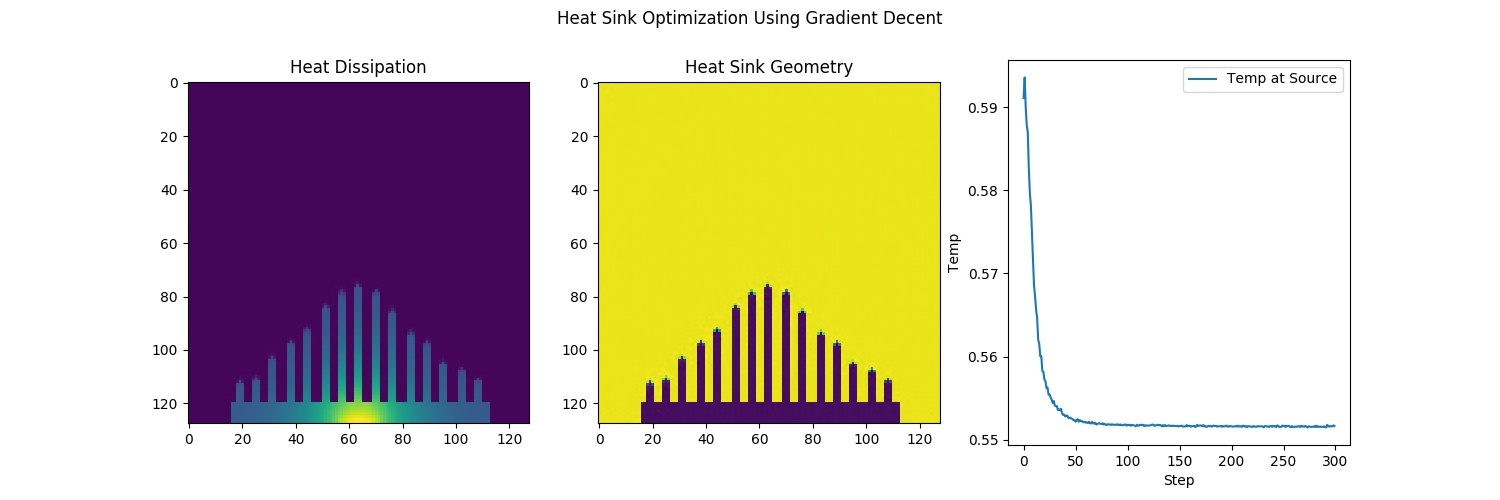
\includegraphics[scale=0.27]{../test/figs/heat_learn_gradient_decent.jpeg}}
\subfigure{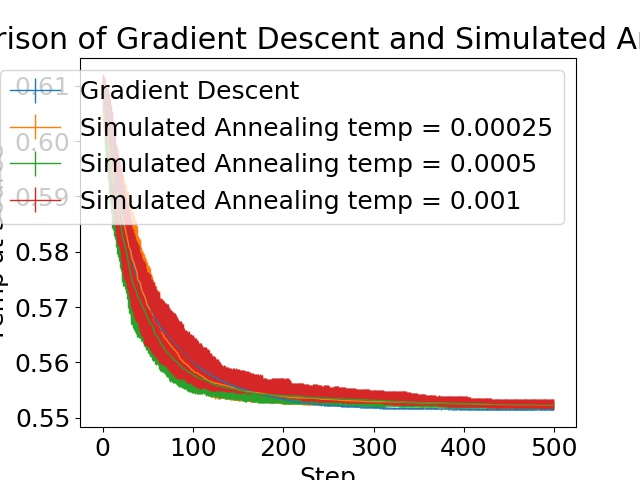
\includegraphics[scale=0.27]{../test/figs/heat_learn_comparison.jpeg}}
\end{center}
\label{heat_sink_optimization}
\caption{A comparison of our gradient decent based method and simulated annealing in optimizing the design of a heat sink. Several starting temperature for the simulated annealing algorithm are provided. Each optimization was performed 40 times from the same starting design and the bars show the standard deviation over these runs.}
\end{figure}

\begin{figure}[h]
\begin{center}
\end{center}
\end{figure}


\subsection{Flow Prediction Accuracy}

Before we move to our final test of designing 2D and 3D airfoils it is worth looking at how accurately our model can predict steady state fluid flow. Our models ability to create designs is dependent on this so testing this is important in understanding its properties. We can also verify our claim of a superior network architecture over previous works and show results indicating this. We omitted this discussion of accuracy from the heat sink problem because we found our model predicted steady state heat distribution so accurately that there was virtually no difference between the simulation and network prediction. In fact the percentage error in predicting the temperature at source was only 0.06 percent different. A figure showing this and other calculations can be found here in the appendix.

The quantities of most interest in our predictions are the forces on the object. These are the values being optimized so being able to predict them accurately is of crushed importance. The forces are calculated from the pressure field by doing a surface integral over the airfoil. This can be done in Tensorflow in a differentiable way by using a 3 by 3 transpose convolution on the binary boundary to determine the surface and surface normals of the object. Then multiplying this with the pressure field and summing to produce the total force. Viscus forces are left out from this calculation as they are relatively small for airfoils. In figure \ref{flow_accuracy} and \ref{flow_accuracy} we see that our model is remarkably accurate in predicting the forces on the airfoil. We also see similar accuracy in predicting maximum velocity. While these values are not much use in our problem we found them to be a strong indicator of how well our model was performing. The reason being that if the network was not learning the flow well it would tend to underestimate these values and average out these values making the flow more uniform. When comparing our network to the previous model we see a clear increase in accuracy. We also visually inspect the flow here and see that predicted flow is very sharp and doesn't have any blurring effects.

\begin{figure}[!t]
\begin{center}
\subfigure{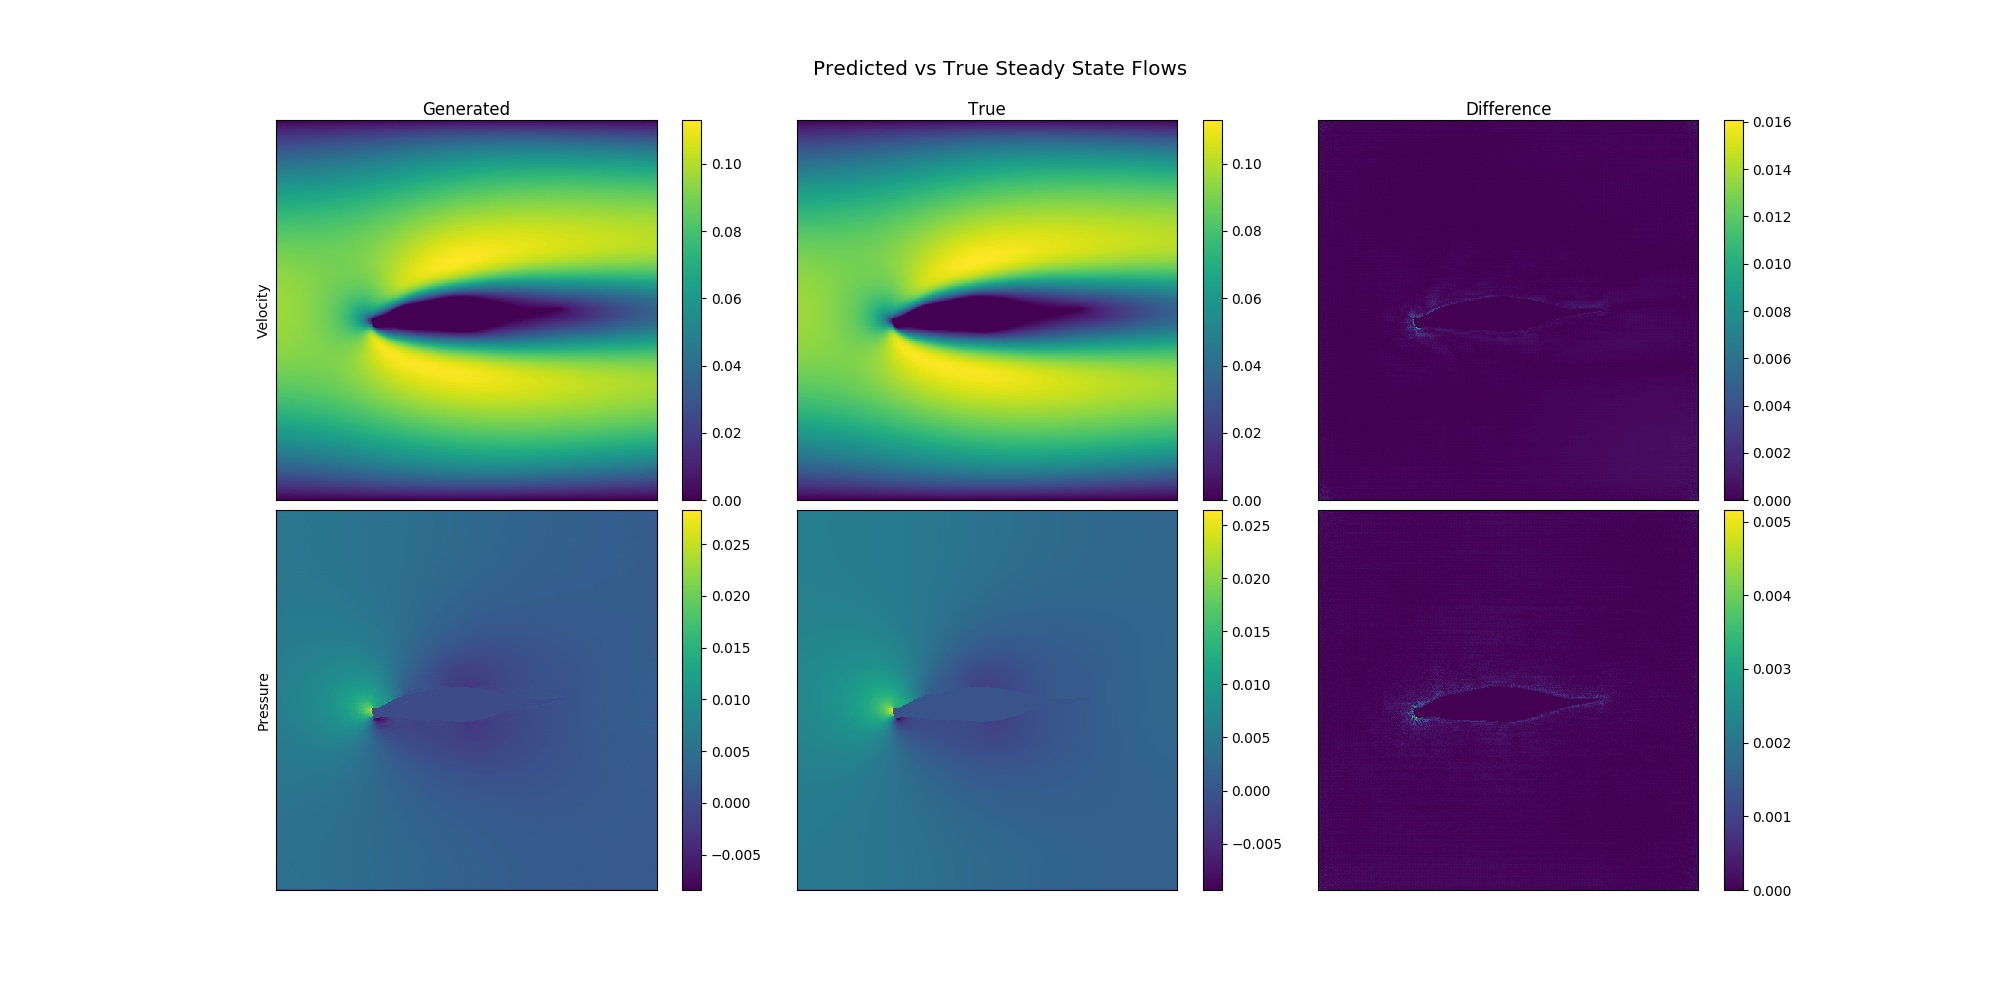
\includegraphics[scale=0.25]{../test/figs/generated_flow_difference.jpeg}}
\subfigure{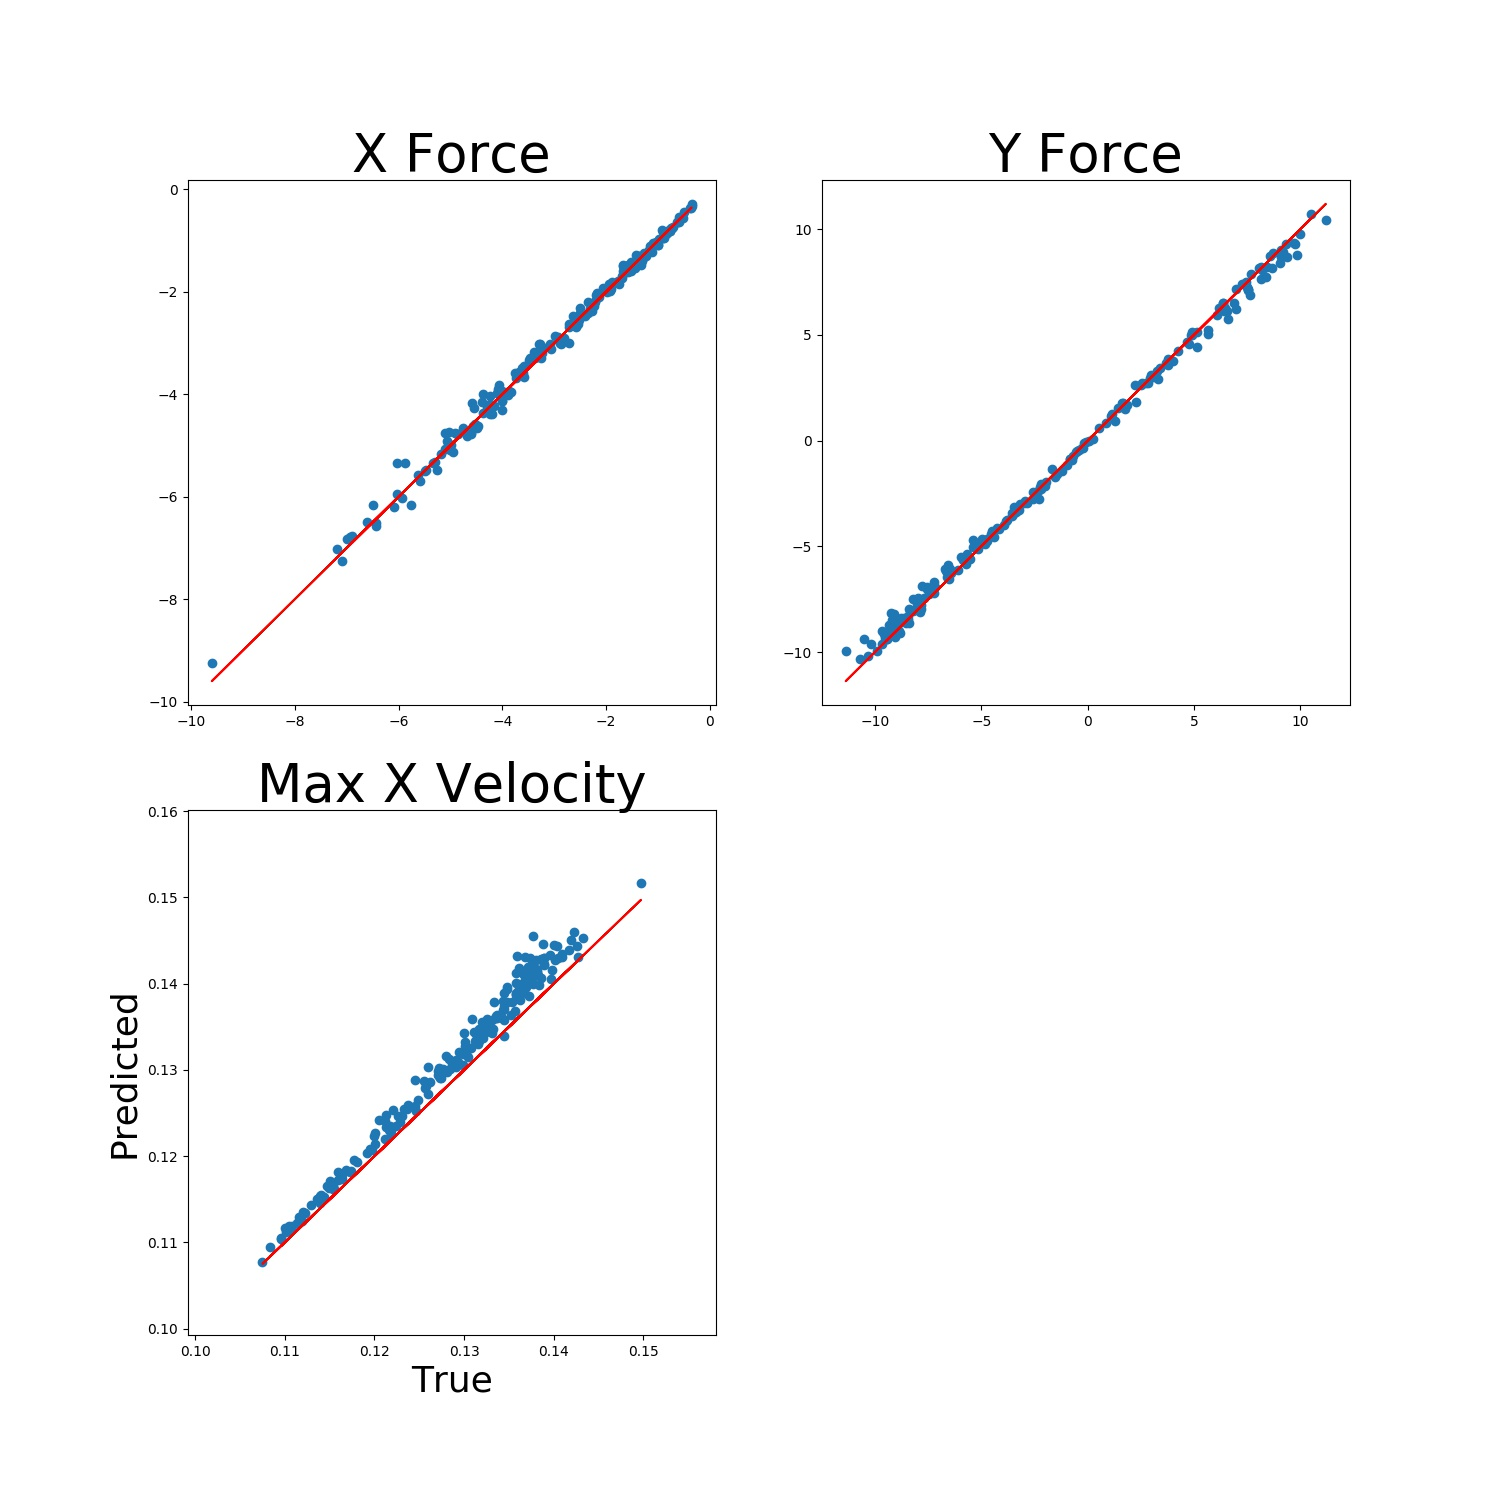
\includegraphics[scale=0.095]{../test/figs/flow_accuracy_2d.jpeg}}
\end{center}
\caption{Comparison of steady state flow predicted by neural network and the lattice Boltzmann flow solver.}
\label{flow_accuracy}
\end{figure}

\begin{figure}[h]
\begin{center}
\end{center}
\caption{Accuracy of the neural network in predicted various quantities.}
\end{figure}

\subsection{Automated Design of 2D and 3D Airfoils}

\begin{figure}[h]
\begin{center}
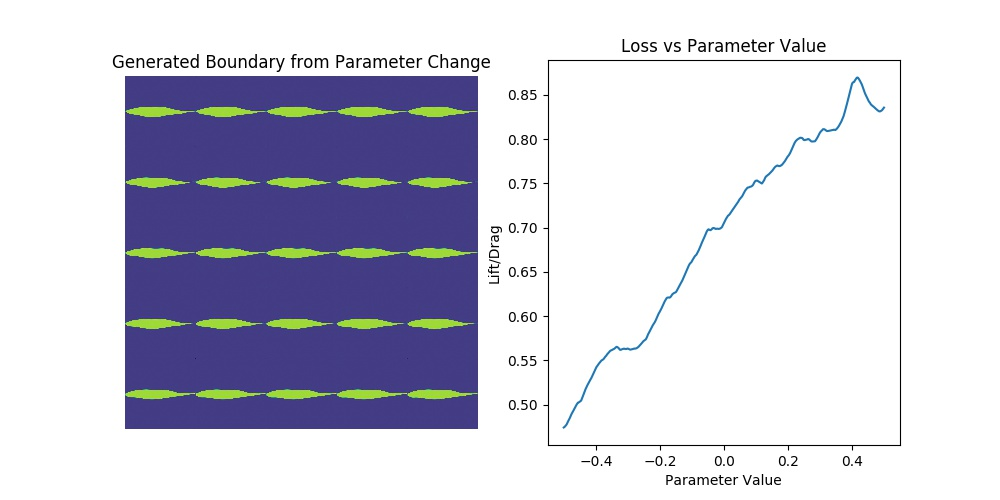
\includegraphics[scale=0.27]{../test/figs/boundary_space_explore.jpeg}
\end{center}
\caption{A look at the design }
\end{figure}

\begin{figure}[h]
\begin{center}
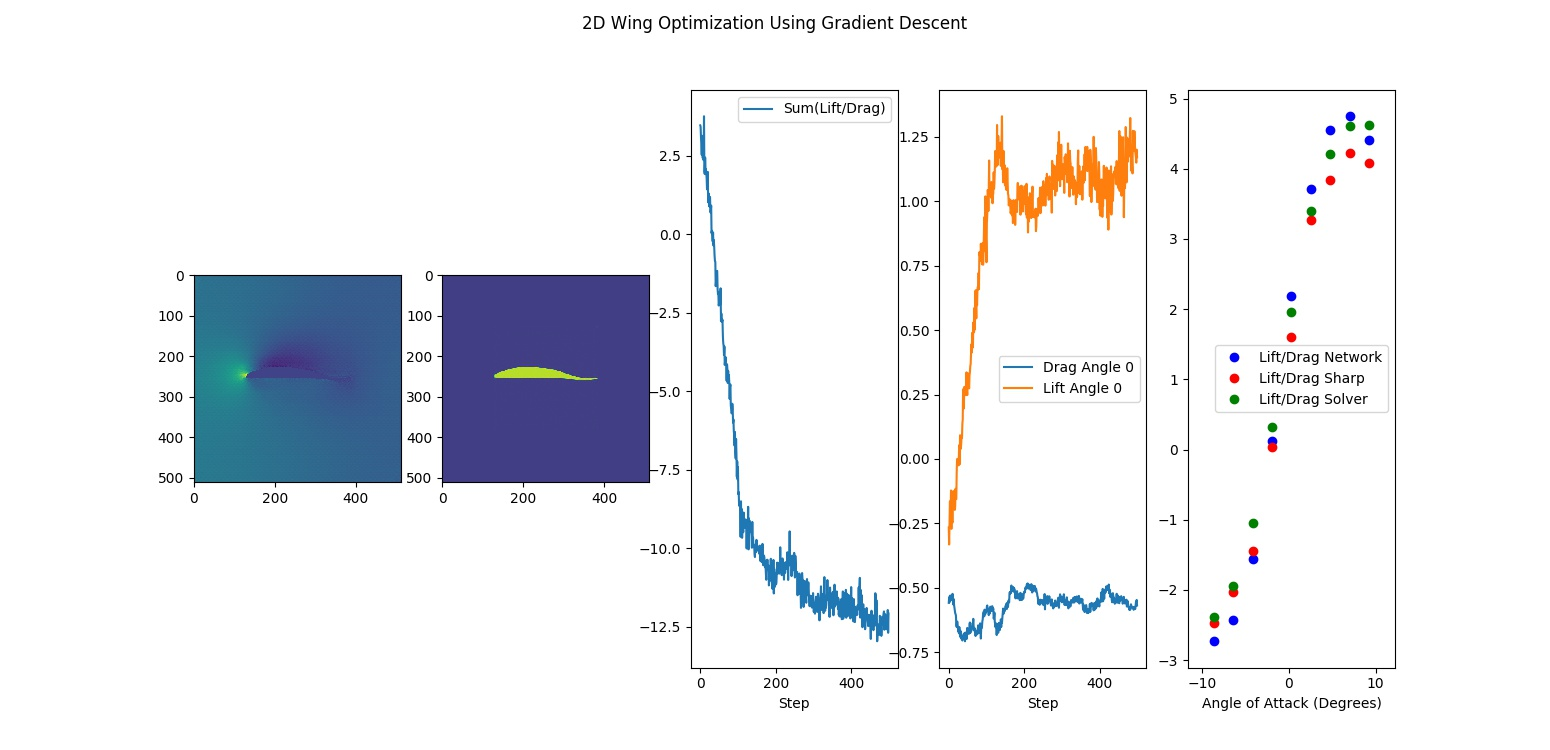
\includegraphics[scale=0.20]{../test/figs/learn_gradient_descent.jpeg}
\end{center}
\caption{Flow}
\end{figure}

\begin{figure}[h]
\begin{center}
\includegraphics[scale=0.20]{../test/figs/wing_3d.jpg}
\end{center}
\caption{Flow}
\end{figure}

\subsection{Comparison of Computation Times}

The central purpose of our approach is to accelerate the automated design process and in this section we attempt to quantify this in real time. The most important quantities are the time to perform a gradient update on the design parameters and the time needed to perform a simulation. We have already briefly discussed the computation time of the heat sink problem and leave this section for the airfoil design problems.

The first comparison we look at is the raw speed of the fluid solver verses the neural network. We found that our flow solver converged to steady state in an average of 60 seconds for the 2D simulation and 300 seconds for the 3D simulation on a Nvidia 1070 GPU. We used the Sailfish library \cite{januszewski2014sailfish} for these simulations as it performed much faster then every other non proprietary lattice Boltzmann based fluid flow library. In particular, we found it superior in speed compared with OpenLB, Palabos, Mechsys, and ASL where only the latter two have naive GPU support. In comparison to our neural network, approximating the steady state flow required only 0.15 seconds with batch size 1 and 0.058 seconds with batch size 16 for the 2D simulation and blaa with batch size 1 and blaa with batch size 10 for the 3D simulation. A more complete list of values can be found in table \ref{computation_table}. While this does represent a significant 1000 times efficiency gain, we do note though that when using the neural network we are only predicting a square box of flow around the object whereas the full simulation works on an area roughly 2 to 4 times larger. There are also methods of accelerating lattice Boltzmann steady state flow calculations that are not explored in this work but which may give around a order or two magnitude speed increase \cite{guo2013lattice} \cite{bernaschi2002computing}. It is also fair to say though that there are many techniques such as blaa that could speed up our neural network computations.

The other computation time that needs to be addressed is how long it takes to compute the gradients. In practice we found that computing the gradient required 3 to 4 times the network evaluation.


\begin{table}[t]
\caption{Sample table title}
\label{computation_table}
\begin{center}
\begin{tabular}{l|lllll}
Batch Size & 1 & 2 & 4 & 8 & 16 \\ \hline 
Flow Net $512^2$ & 0.150 sec & 0.101 sec & 0.077 sec & 0.065 sec & 0.058 sec \\ 
Param Net $512^2$ & 0.083 sec & 0.045 sec & 0.026 sec & 0.015 sec & 0.011 sec \\ 
Learn Step $512^2$ & 0.494 sec & 0.345 sec & 0.270 sec & 0.231 sec & Nan \\ 
Flow Net $144^3$ & 0.826 sec & 0.686 sec & 0.627 sec & 0.623 sec & Nan \\ 
Param Net $144^3$ & 0.195 sec & 0.144 sec & 0.119 sec & 0.106 sec & 0.093 sec \\ 
Learn Step $144^3$ & 3.781 sec & Nan & Nan & Nan & Nan \\ 
\end{tabular}
\end{center}
\end{table}




\section{Conclusion}

In this work we have presented a novel method of design optimization and shown its effectiveness on a variety of tasks. Future work may be to `

\subsubsection*{Acknowledgments}

This work was made possible through the \url{http://aigrant.org} created by Nat Friedman and Daniel Gross. This work would not have be possible without this very genourous support.

\bibliography{iclr2018_conference}
\bibliographystyle{iclr2018_conference}

\section{Appendix}

\begin{figure}[h]
\begin{center}
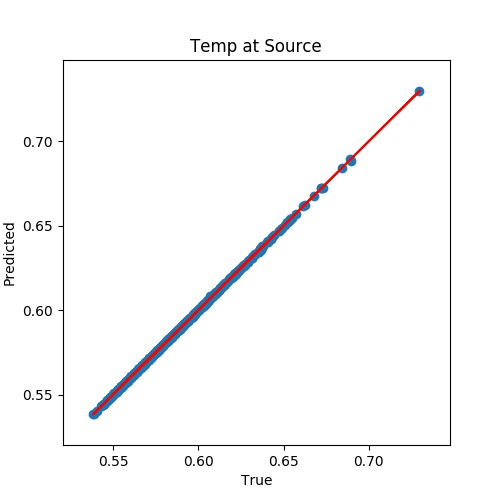
\includegraphics[scale=0.15]{../test/figs/heat_accuracy.jpeg}
\end{center}
\caption{Flow}
\end{figure}


\begin{figure}[h]
\begin{center}
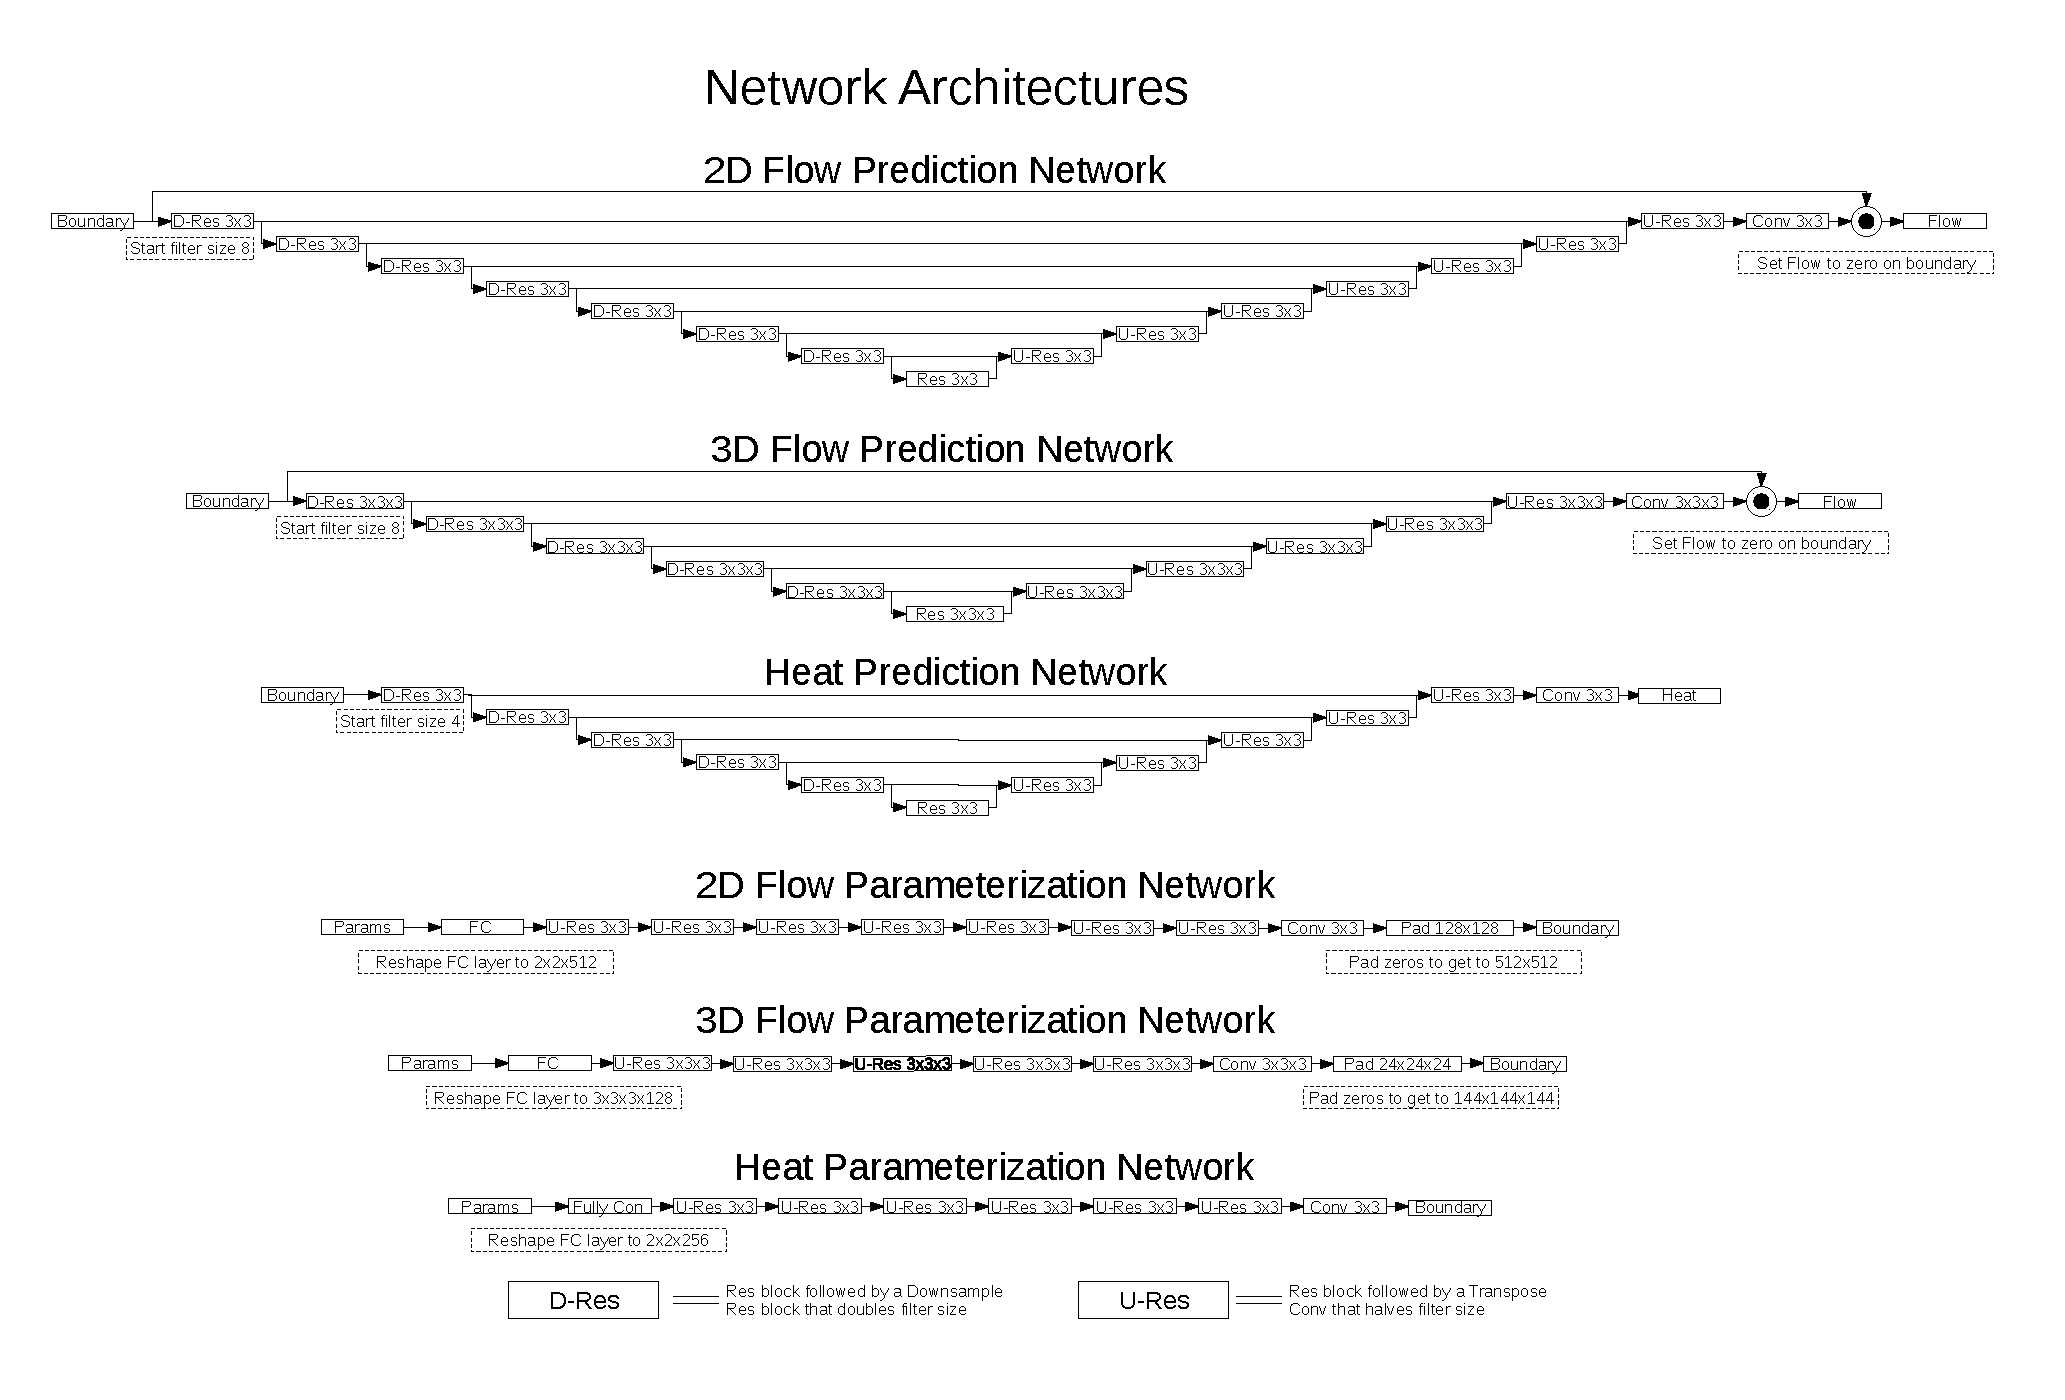
\includegraphics[scale=0.45]{./appendix_flow_net.pdf}
\end{center}
\caption{Flow}
\end{figure}

\end{document}
